\newpage
\begin{figure}
    \begin{center}
        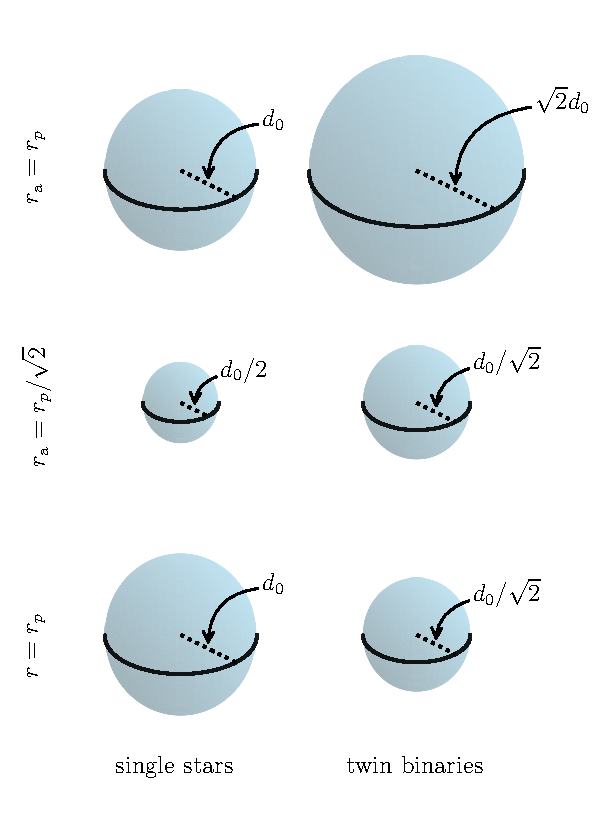
\includegraphics[width=\textwidth]{figures/visualize_volumes.pdf}
    \end{center}
    \caption{
    In Model \#1, we assume all stars have equal mass and luminosity, and that 
    the observer cannot resolve binary systems.
    For single stars (left), at fixed planet size and period, the 
    selected and searchable volumes are then identical.
    Twin binaries (right) are twice as luminous, and so are selected 
    out to a maximum distance $\sqrt{2}\times$ that of single stars 
    (Eq.~\ref{eq:d_sel}).
    However, the diluting light from the twin companion lowers the maximum 
    distance at which a planet can be detected, relative to single stars, by 
    $1/\sqrt{2}$ (Eq.~\ref{eq:d_det_i}).
    }
    \label{fig:model_1_volumes}
\end{figure}


\begin{figure}
    \begin{center}
        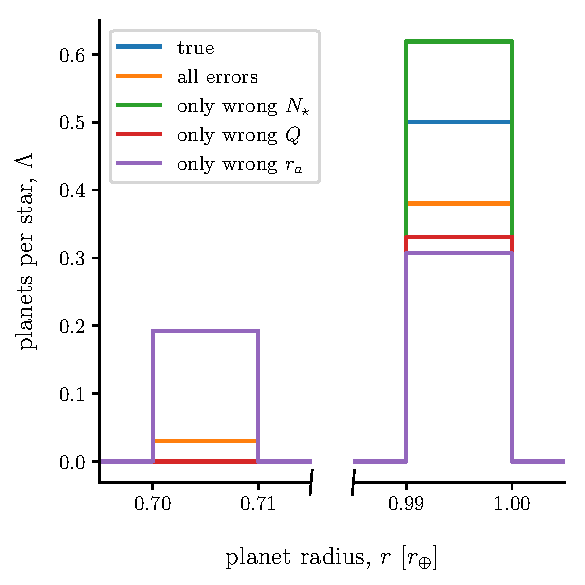
\includegraphics[width=\textwidth]{figures/errcases_rate_density_vs_radius_model_1_brokenx.pdf}
    \end{center}
    \caption{
    Inferred planet occurrence rates as a function of planet radius in Model 
    \#1.
    This model has fixed stars, fixed planets, and twin binaries.
    If the true planet radius is $r_p$, all planets 
    detected in binaries will have apparent radii $r_a = r_p/\sqrt{2}$.
    Only 1 in 8 selected binaries is actually searchable (see 
    Sec.~\ref{sec:model_1}).
    To help illustrate the individual effects of errors, we 
    separated them:
    ``only wrong $N_\star$'' means the only error is an incorrectly assumed 
    number of selected stars;
    ``only wrong $Q$'' means the only error is an incorrectly assumed 
    detection efficiency (including both miscalculated transit probabilities 
    and 
    fraction of selected stars that are searchable);
    ``only wrong $r_a$'' means the only error is misinterpretation of 
    planetary radii, due to both transit depth dilution and also wrongly 
    assumed host star radii.
    }
    \label{fig:errcases_model_1}
\end{figure}

\begin{figure}[!tb]
    \centering
    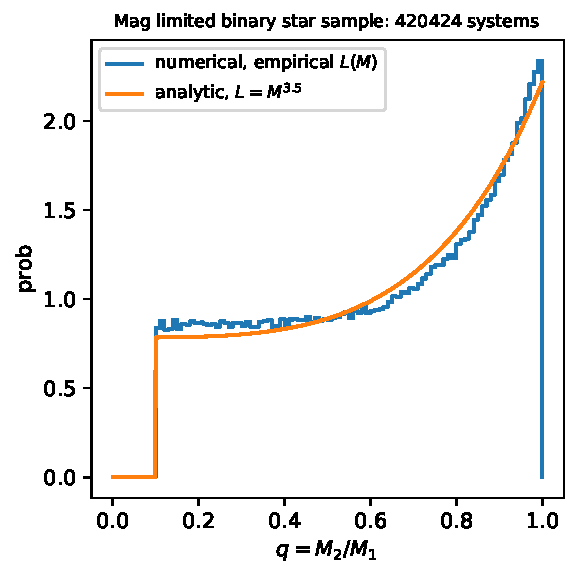
\includegraphics[width=\textwidth]{figures/q_distribn_mag_limited.pdf}
    \caption{
    The distribution of the mass ratio for a magnitude limited sample of 
    binary stars. The underlying mass ratios are drawn from a uniform 
    distribution in a volume-limited sample, quite similar to that of Raghavan 
    et al. (2010)'s Fig. 13.
    The entire bias can be understood analytically (Eq.~\ref{eq:model_2_p_2},
    with $\gamma=0$).
    The numerical comparison uses a realistic empirical mass-luminosity 
    relation rather than $L=M^{3.5}$, found by fitting main sequence dwarf 
    mass luminosity data compiled from Torres et al. [2009] and Benedict et 
    al. [2016].
    }
    \label{fig:q_distribn_mag_limited}
\end{figure}


\begin{figure}[!tb]
    \centering
    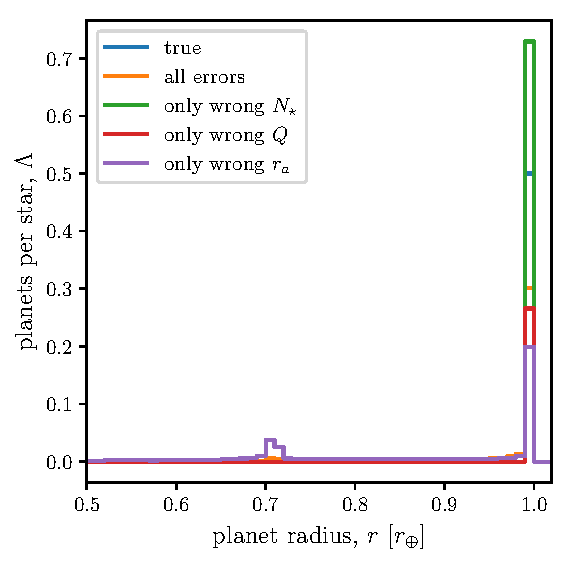
\includegraphics[width=.7\textwidth]{figures/errcases_rate_density_vs_radius_model_2.pdf}
    \caption{
    Inferred planet occurrence rates as a function of planet radius in Model 
    \#2.
    This model has fixed planets and primaries, but varying secondaries.
    }
    \label{fig:errcases_model_2_linear}
\end{figure}

\begin{figure}[!tb]
    \centering
    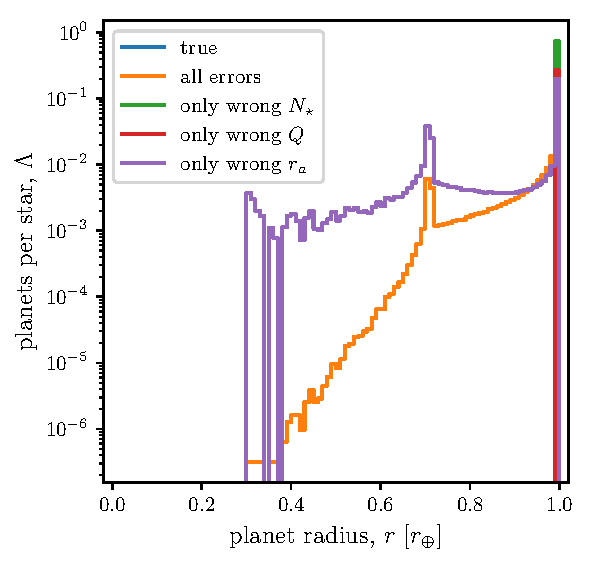
\includegraphics[width=.7\textwidth]{figures/errcases_rate_density_vs_radius_logs_model_2.pdf}
    \caption{
    Same as Fig.~\ref{fig:errcases_model_2_linear}, but with logarithmic 
    $y$-axis, and different $x$ scale.
    }
    \label{fig:errcases_model_2_log}
\end{figure}

\begin{figure}[!tb]
    \centering
    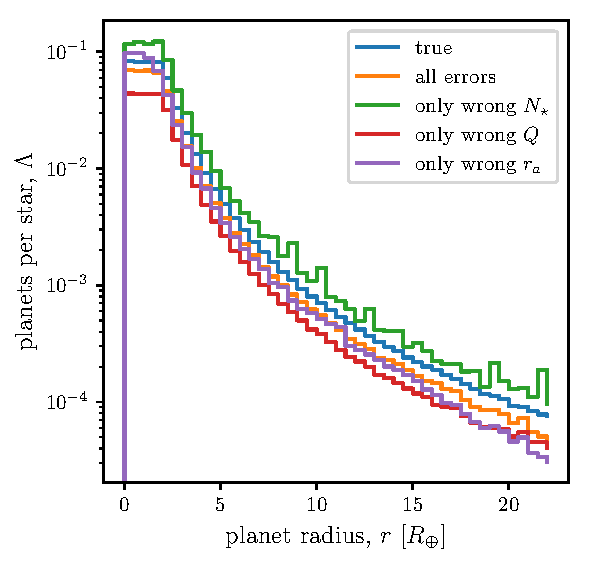
\includegraphics[width=\textwidth]{figures/errcases_rate_density_vs_radius_logs_model_3.pdf}
    \caption{
    Inferred planet occurrence rates as a function of planet radius in Model 
    \#3.
    This model has fixed primaries and single stars, but varying 
    secondaries.
    The true planet radius distribution is a power law with exponent $-2.92$ 
    above $2R_\oplus$, below which it is uniform (e.g., Howard et al., 
    2012).
    }
    \label{fig:errcases_model_3_log}
\end{figure}

\begin{figure}[!tb]
    \centering
    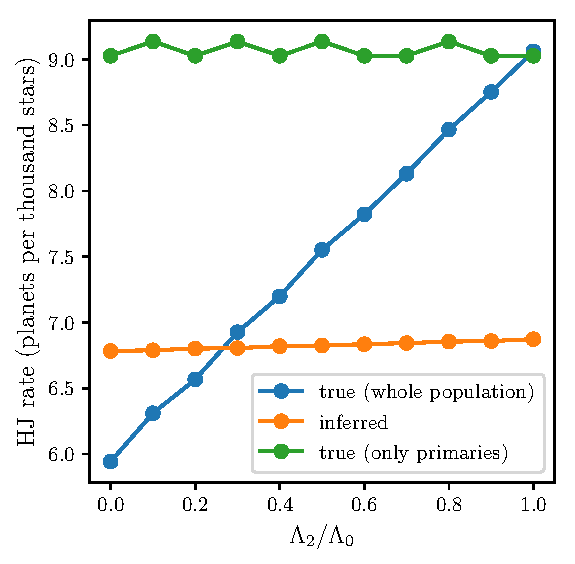
\includegraphics[width=.9\textwidth]{figures/HJ_correction_inputrate_vs_HJratevalues.pdf}
    \caption{
    $\Lambda_i$ is the occurrence rate integrated over all possible phase 
    space for the $i^{\rm th}$ system type. $\Lambda_2/\Lambda_0=1$ 
    corresponds to an equal number of planets per secondary as per single star;
    $\Lambda_2/\Lambda_0=0$ corresponds to secondaries not having any planets.
    In our Model \#3, though the true HJ occurrence rate 
    (Eq.~\ref{eq:occ_rate}) is highly dependent on $\Lambda_2$, 
    the inferred rate hardly depends on whether secondaries have HJs.
    This means that the ``correction factor'' between the inferred rate and 
    the true rate around single stars is underestimated by a multiplicative 
    factor of $\approx1.3$, independent of the HJ rate around secondaries.
    The ``HJ rate'' is the summed rate from     
    Fig.~\ref{fig:errcases_model_3_log} above $8r_\oplus$.
    }
    \label{fig:HJ_correction_inputrate_vs_HJratevalues}
\end{figure}

\begin{figure}[!tb]
    \centering
    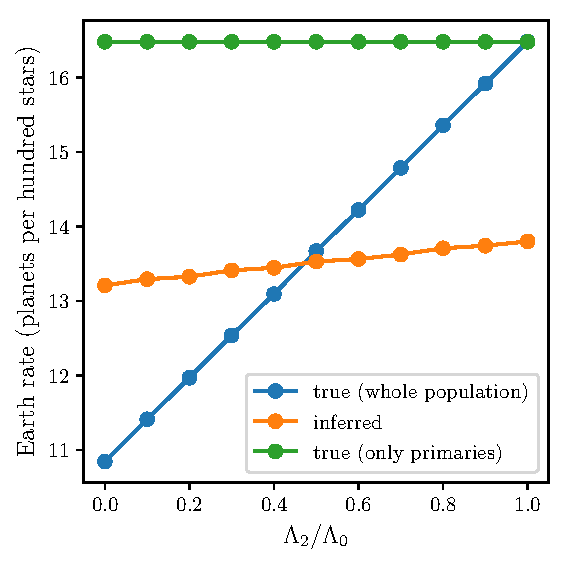
\includegraphics[width=.9\textwidth]{figures/earth_inputrate_vs_etaearthratevalues.pdf}
    \caption{
        Same as Fig.~\ref{fig:HJ_correction_inputrate_vs_HJratevalues}, but 
        for Earth-sized planets.
        The absolute values given on the $y$-axis found by summing the rate 
        from Fig.~\ref{fig:errcases_model_3_log} for planetary radii from 
        $0.5$ to $1.5r_\oplus$ (this is a toy model, and they do not reflect 
        an actual determination of $\eta_\oplus$).
        The relative values show that the inferred rate for Earths is roughly 
        independent of the occurrence rate (integrated over all radii) around 
        secondaries.
        However, it is systematically lower than the true rate around single 
        and primary stars, by $\approx 20\%$.
    }
    \label{fig:earth_inputrate_vs_etaearthratevalues}
\end{figure}


%\begin{figure}[!b]
%    \begin{center}
%        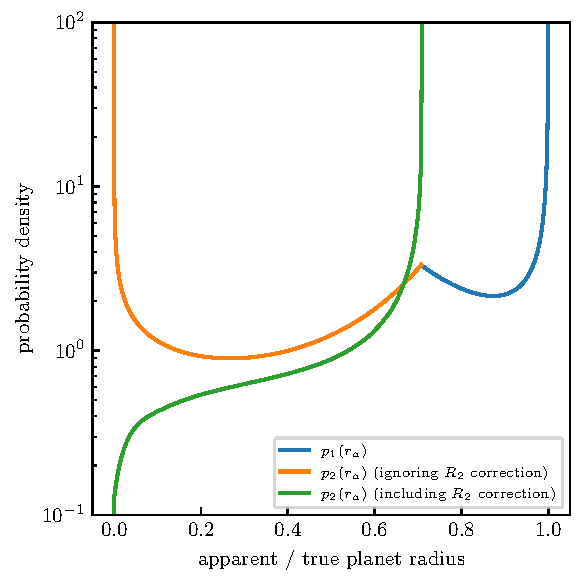
\includegraphics[width=.9\textwidth]{figures/prob_r_a.pdf}
%    \end{center}
%    \caption{Model \#2 (Sec.~\ref{sec:model_2}): 
%    probability of observing an apparent radius $r_a$ given a 
%    planet orbiting the primary, $p_1(r_a)$, or the secondary, $p_2(r_a)$ of 
%    a 
%    binary system.
%    The true planet radius is fixed~--~a delta function centered on ``1''.
%    This plot takes $\alpha=3.5, \beta=0$, for $\alpha$ the exponent in 
%    the mass-luminosity relation $L \propto M^\alpha$, and $\beta$ the 
%    exponent in the distribution of mass ratios in a volume-limited sample.
%    Each distribution is separately normalized.
%    }
%    \label{fig:model2_prob_r_a}
%\end{figure}
